\documentclass[a4paper,12pt]{article} 


\usepackage[T2A]{fontenc}			% кодировка
\usepackage[utf8]{inputenc}			% кодировка исходного текста
\usepackage[english,russian]{babel}	% локализация и переносы


% Математика
\usepackage{amsmath,amsfonts,amssymb,amsthm,mathtools} 

\usepackage{gensymb}	
\usepackage{wasysym}

% Картинки
\usepackage{graphicx}
\graphicspath{{images/}}

%Заговолок
\usepackage[left=2cm,right=2cm,
    top=2cm,bottom=2cm,bindingoffset=0cm]{geometry}

\usepackage{titling}


\author{Петров Артём Антонович, группа 721}
\title{"Лабораторная работа № 2.4.1 "Определение теплоты испарения жидкости"}
\date{\today}

\begin{document} % начало документа

\begin{minipage}[t][8cm]{\textwidth}
\maketitle
\end{minipage}


\textbf{Цель работы:} Вычисление теплоты испарения жидкости с помощью уравнения Клапейрона-Клаузиуса.
\bigskip

\textbf{Оборудование:} термостат, герметичный сосуд с исследуемой жидкостью и манометром, отсчётный микроскоп.
\bigskip

\textbf{Теория}
\bigskip

Уравнение Клапейрона-Клаузиуса:

\begin{equation}\label{eq:klap-klauz}
\frac{dP}{dT} = \frac{L}{T (V_2 - V_1)}
\end{equation}

Где $P$ - давление пара жидкости при температуре $T$. $T$ - абсолютная температура жидкости (и пара). $L$ - теплота испарения жидкости. $V_2$ и $V_1$ - объёмы пара и жидкости соответственно. Величины удельные (на 1 моль).

В нашем опыте можно будет принебречь $V_1$ по сравнению с $V_2$, так как удельный обьём жидкости много меньше удельного обьёма пара при наших порядках температур и давления (в сосуде давление газа(паров) ниже атмосферного). В дальнейшем будем вместо $V_2$ писать $V$.

Так как сосуд с жидкостью запаян, а воздух был выкачан из него перед герметизацией, над житкостью находится насыщенный пар.

Он подчиняется уравнению Ван-дер-Ваальса:

\begin{equation}\label{eq:real-gas}
\bigg(P + \frac{\alpha}{V^2}\bigg)(V-b) = RT
\end{equation}
 
 Однако, при наших диапазонах $P$ и $T$, $b \sim V_1 << V_2$ и $\alpha/V^2 << P$. Таким образом получаем уравнение Клапейрона:
 
\begin{equation}\label{eq:ideal-gas}
PV = RT
\end{equation}

Откуда получаем:

\begin{equation}\label{eq:ideal-gas2}
V = \frac{RT}{P}
\end{equation}
 
Подставляя \ref{eq:ideal-gas2} в \ref{eq:klap-klauz} и выражая $L$ получаем:

\begin{equation}\label{eq:final-eq}
L = \frac{RT^2}{P}\frac{dP}{dT} = -R\frac{d(lnP)}{d(1/T)}
\end{equation}

Измеряя $T$ термостатом и $P$ c помощью манометра с микроскопом и проведя соответствующие вычисления можно получить зависимость $ln(P)$ от $1/T$. По ней можно найти $dP/dT$ и вычислить $L$ по \ref{eq:final-eq}.
\bigskip

\textbf{Установка:}
\medskip

На схеме \ref{schema} представлена эксперементальня установка. 

\begin{figure}[ht]
\centering
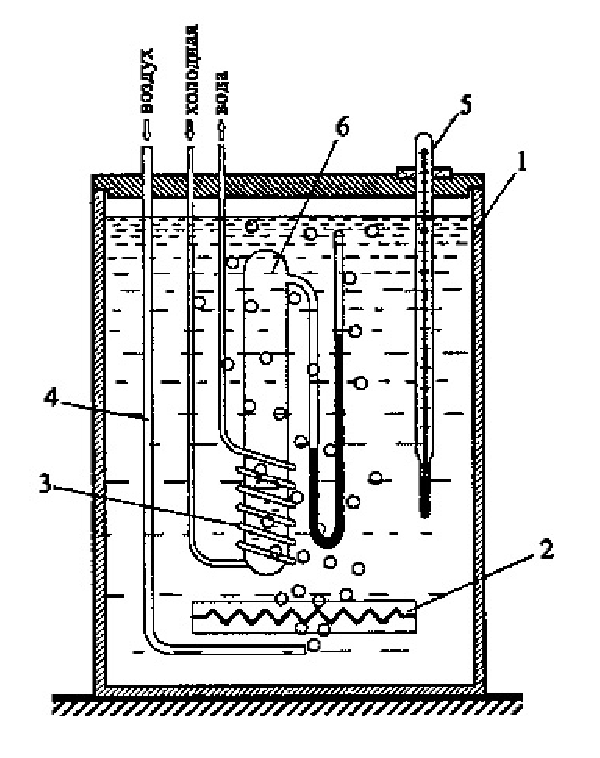
\includegraphics[width=80mm]{schema.eps}
\caption{Схема установки: 1 - термостат с системой контроля температуры воды (2,3 и 4); 5 - термометр; 6 - герметичный сосуд с исследуемой жидкостью}\label{schema}
\end{figure}

Показания манометра снимаются с помощью микроскопа.

Важно помнить, что термометр измеряет не температуру исследуемой жидкости (и её паров) $T$, а температуру термостата, которая  $\sim T$ только при медленном нагреве. Для проверки того, что в нашем эксперименте изменение температуры достаточно медленное снимем зависимость $P$ от $T$ как при нагреве, так и при охлаждении. Если они совпадут, то скорость изменения $T$ выбрана верно.
\bigskip

\textbf{Ход работы:}
\bigskip

Заметим, что поверх одного из столбиков ртути в манометре есть конденсат жидкости. Необходимо будет учитывать его вклад в показания манометра при измерении давления.

Снимаем значения $h_{base}$ - высоту нижнего столбика ртути, $h_{hidrargium}$ - высоту верхнего столбика  и $h_{spirit}$ с помощью манометра и микроскопа. Давление паров над жидкостью найдём по формуле: 

\begin{equation}\label{eq:p-from-h}
P = ((h_{hidrargium} - h_{base})*\rho_{hidrargium} - (h_{spirit} - h_{base})*\rho_{spirit})*g
\end{equation}

Температуру будем измерять напрямую с помощью термометра.
\medskip

1) Снимем данные для комнатной температуры.

2) Повысим температуру на 2 градуса и подождём пока термостат нагреется и установится тепловое равновесие.

3)Снимем данные.

4)Повторим пункты 2 - 3.

5)Теперь отключим термостат и снимем данные для уменьшения температур.( с помощью добавления в термостат холодной водопроводной воды и слива излишков)

6)Вычислим зависимость $ln(P)$ от $1/T$.

7)По формуле \ref{eq:final-eq} используя полученную зависимость найдём $L$.
\bigskip

\textbf{Записи из журнала:}
\bigskip

Выполним пункты 1-4 до достижения температуры в 38 градусов. Установления теплового равновесия будем ждать $ \sim 1 $ минуту.

Затем выполним пункт 5 до достижения температуры $ \sim24\degree $ . Заметим, что очень трудно добиться чёткого шага в $ 2\degree $ при понижении температуры указанным методом.


\begin{figure}[ht]
\centering
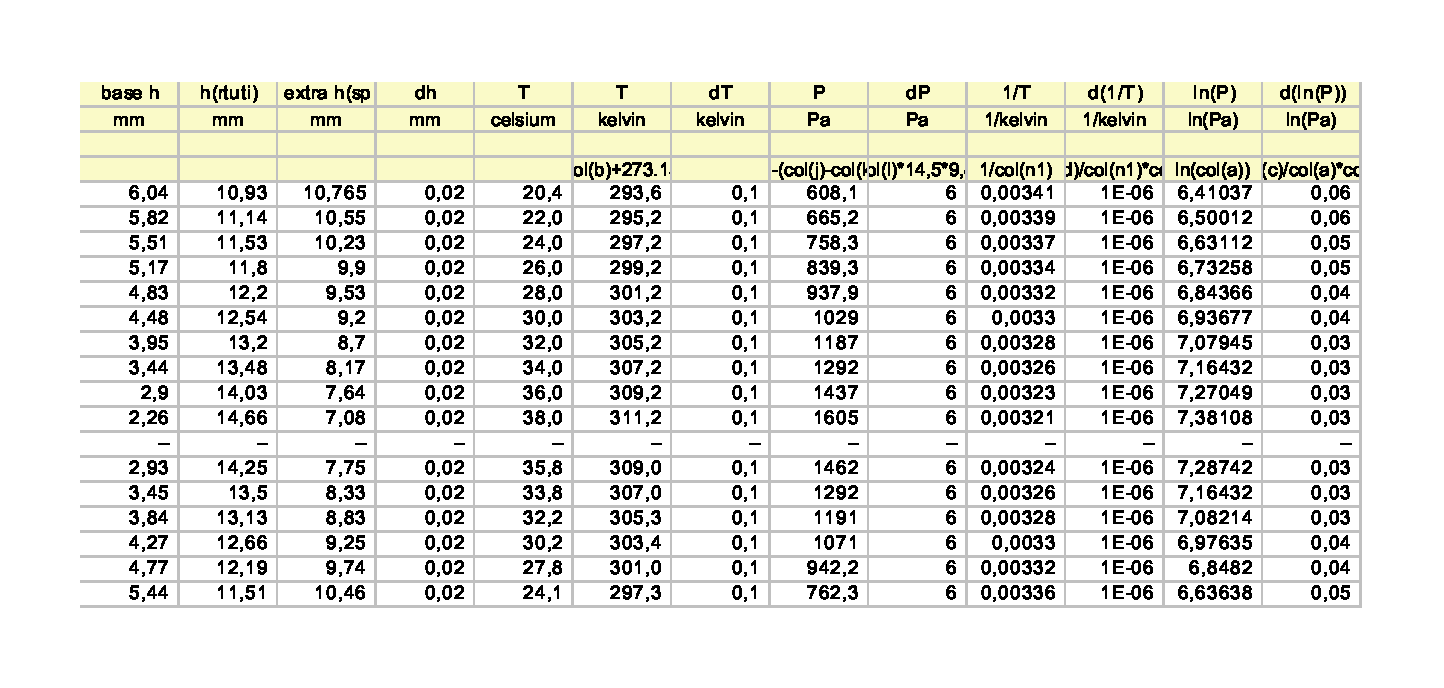
\includegraphics[width=170mm]{table.eps}
\caption{Таблица результатов измерений и их обработки. Обозначения: Измеряемые величины: $ T $ - температура воды в термостате, $ h_{base} $ - высота более низкого столба ртути, $ h_{extra} $ - высота столбика спирта над более низким столбиком ртути, $ h $ - высота более высокого столбика ртути; Вычисляемые величины: $ P $ - давление пара. }\label{lab_table}
\end{figure}

\begin{figure}[ht]
\centering
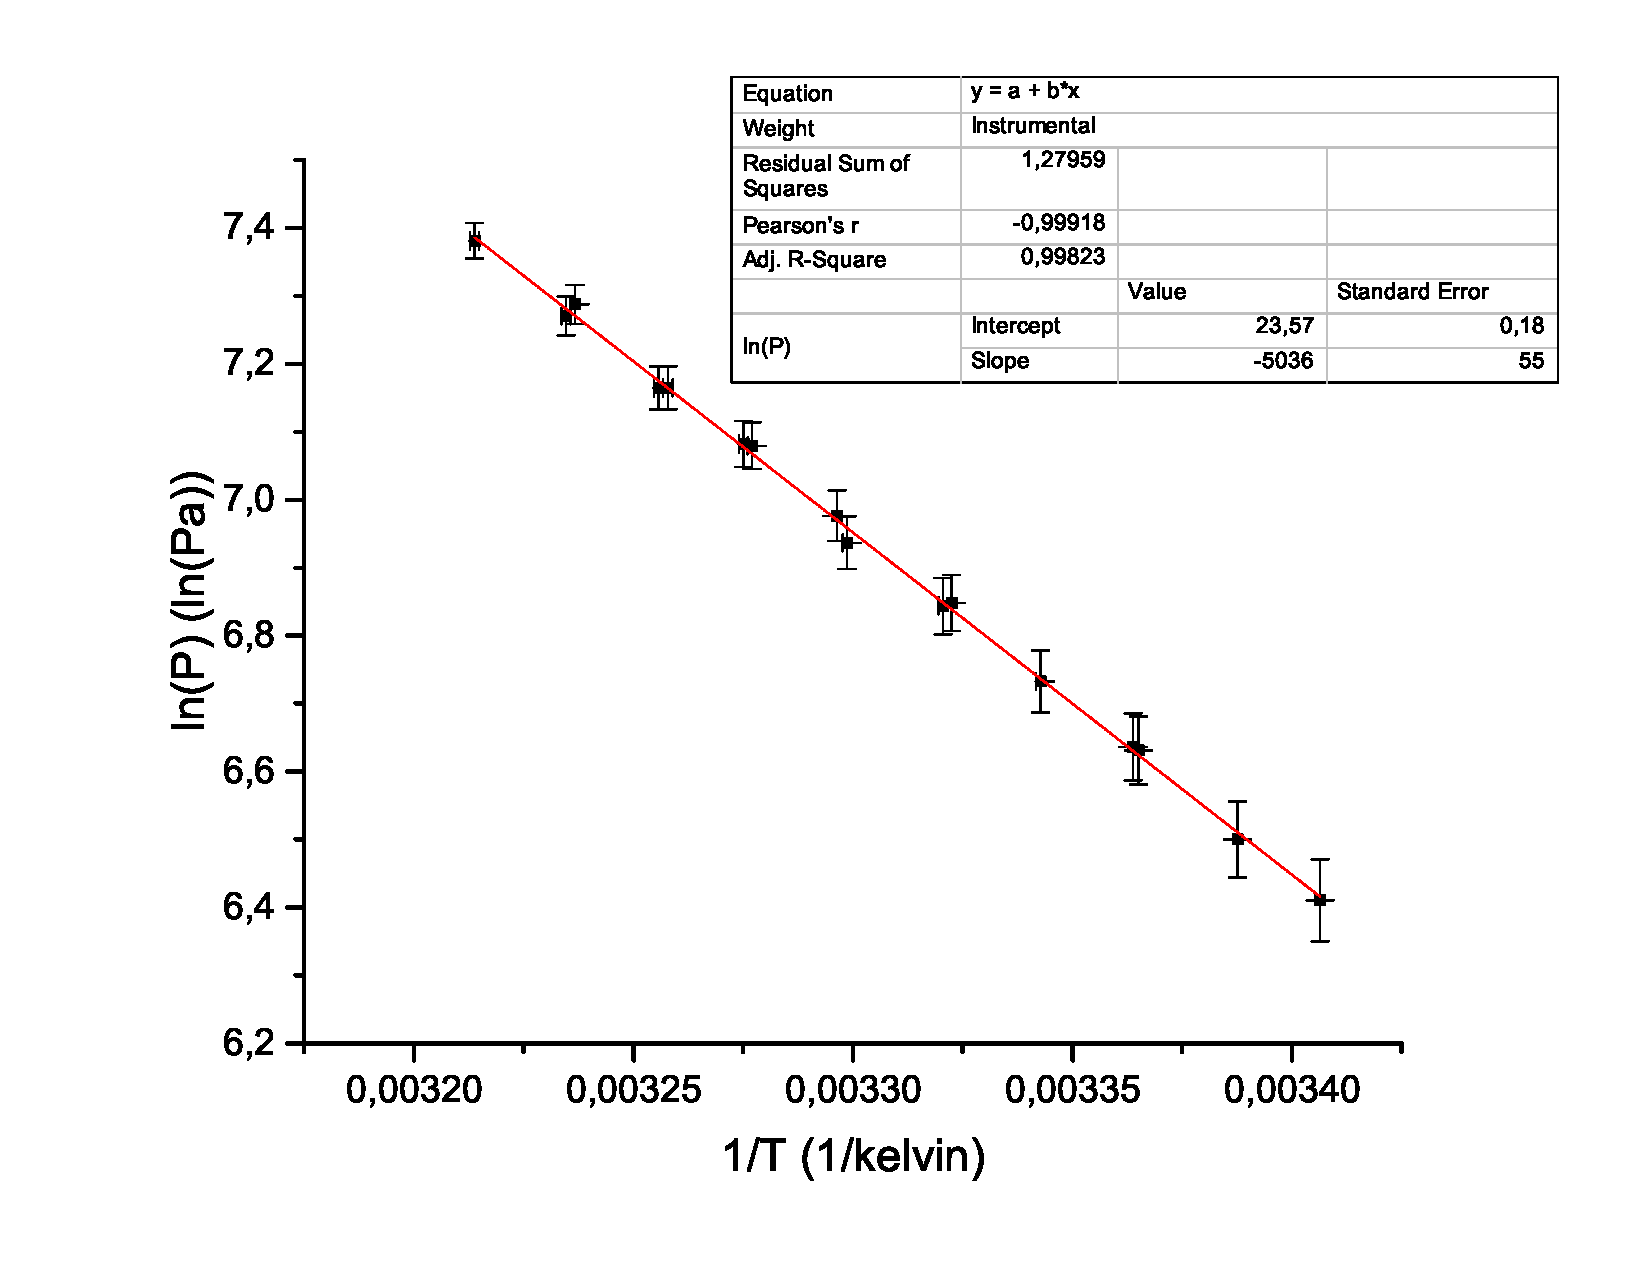
\includegraphics[width=170mm]{graph1.eps}
\caption{График}\label{graph_1}
\end{figure}

Дальше найдём коэффициент наклона линейной зависимости $ ln(P)(1/T) $ и рассчитаем $L$ по формуле \ref{eq:final-eq}.

\bigskip\bigskip\bigskip\bigskip\bigskip\bigskip\bigskip\bigskip\bigskip\bigskip\bigskip\bigskip

Получено значение $L = (41900 \pm 500) \frac{J}{mole}$.
\bigskip

\textbf{Итог:}
\bigskip

\begin{equation}\label{eq:result}
L = (41900 \pm 500) \frac{J}{mole}
\end{equation}

Как видно из графика \ref{graph_1} зависимость идеально ложится на прямую, подтверждая предсказания уравнения Клапейрона-Клаузиуса и наших предположений относитьельно малости величин ($b \sim V_1 << V_2$ и $\alpha/V^2 << P$). 

Полученное значение \ref{eq:result} не сильно отличается от табличного значения $L_{table} = 40700 \frac{kJ}{mole}$ при атмосферном давлении. Хорошим объяснением того, что полученное значение ниже табличного является то, что давление в герметичном сосуде ниже атмосферного, а известно, что при понижении давления, $L$ растёт.
 
\end{document} % конец документа